% !TeX root = ../main.tex

\chapter{基于值流图的整型变量关系分析与缺陷检测}

本章介绍基于值流图的整型变量关系分析与缺陷检测方法,该方法的核心是快速、自动化的从代码中抽取出程序语义,建立程序实现与需求之间的关系,帮助开发人员理解程序进行需求确认。

本章结构安排如下:\ref{sec:值流图引言}小节简要归纳了当前程序理解技术,提出本章工作的实际意义与必要性;\ref{sec:值流图案例分析}小节通过一个需求与实现的例子具体介绍了本章工作如何帮助开发人员快速进行软件确认;随后\ref{sec:值流图程序理解方法}小节具体介绍了算法的原理与实现方法,并于\ref{sec:值流图评估与结果}小节进行了实验验证。\ref{sec:值流图总结}小节最后对本章工作做了总结。

\section{引言}
\label{sec:值流图引言}

软件验证与确认是软件研发过程中十分重要的步骤。其中,对软件确认过程来说,人们除了使用测试的手段逐条对软件行为进行验证以外,最常用的手段便是在理解程序代码的基础上对程序是否符合软件需求做判断。但是,在条件分支众多、代码逻辑复杂的情况下,现有工具很难帮助用户理清程序输入输出变量之间的关系。文章\inlinecite{maalej2010can}指出,约25\%的代码维护工作流程是发现问题-修改-再验证的,同时,大量的开发者通过假设并验证程序的行为来理解软件\cite{maalej2014comprehension}。因此,若使用一种算法(工具)帮助开发者快速准确地抽取程序语义将会大大减少程序理解相关工作时间。

程序理解\cite{boysen1979factors, sackman1968exploratory}领域以往的研究工作主要基于程序切片技术、程序标记技术以及执行可视化技术。

程序切片技术\cite{binkley1996program}本质上是一种代码拆解技术。它通过剔除与指定变量不相关的代码语句,一定程度上减少了用户的代码阅读量。但是由于其并未能给出更上层的程序语义,用户仍需要阅读源码以获取知识。与之相反,程序标记技术\cite{sulir2017labeling}通过在源码上附加辅助信息的方式来帮助用户理解代码。现有工具可提供的辅助信息多种多样,但本质上用户仍要理解代码逻辑,并不能显著提升程序理解速度。执行可视化工具使用动态分析获取程序的执行信息并将之可视化,为了达到分析目的,工具将不同执行过程信息加以融合。其缺点是当程序逻辑复杂时,可视化的效果会变差,且需要为其配置程序运行环境,具有上手难度。 

本章中,我们提出了一种基于精确值流图(Value Flow Graph,简称VFG)的自动化程序静态分析算法,该算法通过使用指针分析得到内存模型,基于内存模型构造VFG,并进一步分析得到VFG上的程序语义。

本方法是纯静态分析方法,不依赖于程序的具体执行路径,拥有较好的完备性。分析结果可用于开发人员进行程序理解和需求确认,也可以用于自动化的缺陷分析。

\section{案例分析}
\label{sec:值流图案例分析}

程序理解往往是软件研发、软件验证与维护工作中耗时最大的工作内容。本节选取了某机动车变速器控制逻辑的部分软件需求与代码实现作为分析案例来介绍本章所述算法。

\begin{figure}[H]
	\centering
	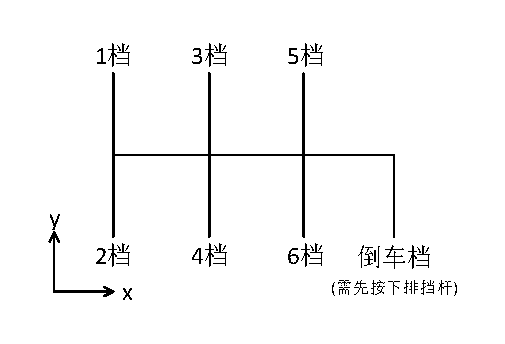
\includegraphics{变速器排挡杆.pdf}
	\caption{变速器排挡杆}
	\label{fig:gearLever}
\end{figure}

该控制逻辑应用于六档变速杆,支持下压式倒挡,其档位映射如图\ref{fig:gearLever}所示。现要求实现相关函数完成图\ref{fig:gearLever}所示控制逻辑,代码应遵循如下要求:

\begin{enumerate}
	\item 该函数应接受4个参数:$ x $、$ y $、$ diverse $和$ oldGear $,根据参数计算出档位值$ gear $并返回;
	\item 返回的档位值$ gear $的取值集合为$\left\{0, 1, 2, 3, 4, 5, 6, -1, -2\right\}$。其中1-6为前进档,-2为倒车档;
	\item $ x $为变速器挡杆在水平方向上的行程。当取值在[0, 380)区间时,表示1或2档;当取值在[380, 690]区间时,表示3或4档;当取值大于690时,表示5、6或-2档(倒车档);
	\item  $ y $为变速器挡杆在竖直方向上的行程。当取值在[0, 160)区间时,档位的可能取值为2、4、6档和-2档;当取值在[160, 780]区间时,档位的可能取值为0或-1(要求下压挡杆);当取值大于780时,档位的可能取值为1、3和5档;
	\item $ diverse $为倒挡信号,当下压变速器挡杆时$ diverse $值为1,否则为0;
	\item $ oldGear $的取值为本次变速器挡杆操作前的档位取值。
\end{enumerate}

\begin{lstlisting}[label=code:gearLever,caption=变速器档位控制的一个函数实现]
int calculateGear(uint x, uint y, uint diverse, int oldGear)
{
	int gear = 0;
	if (y < 160) {
		if (x < 380)
			gear = 2;
		else if (x > 690)
			gear = 6;
		else
			gear = 4;
	}
	else if (y > 780) {
		if (x < 380)
			gear = 1;
		else if (x > 690)
			gear = 5;
		else
			gear = 3;
	}
	if (diverse) {
		if ((gear == 6) && ((oldGear == -1 || oldGear == -2)))
			gear = -2;
		else if (gear == 0);
			gear = -1;
		}
	return gear;
}
\end{lstlisting}

如代码\ref{code:gearLever}所示为上述需求所对应的一个函数实现。当参数取值情况多种多样、条件分支复杂时,开发人员将难以直观的获取到输入输出之间的关系。例如,在需求文档中,档位值为6的条件是$  (x > 690 ∧ y < 160 ∧ (diverse = 0 ∨ (oldGear ≠ -1 ∧ oldGear ≠ -2))) $,但开发者很难直观从代码中获取到相应的控制条件,只有通过表达式分析,才可以自动从代码中得知。试想,如果纯人工的完成这样的行为,不仅费时费力还可能出现条件遗漏和边界条件错误等情况。
更重要的是,因为人工操作的不稳定,很难抓住需求和代码实现之间的微小差异。例如,在以上代码中实际存在了一个很严重的语义问题,导致在$ diverse ≠ 0 $的情况下代码执行与预期不符。即使有完整的需求文档与源代码,没有工具支持的情况下对其进行一致性确认也是十分困难的事情。
本章所述工具可以帮助解决以上问题。如表\ref{tab:summaryFromGearLever}的1、3列所示为期望的返回值与控制逻辑,而实际代码的行为如表\ref{tab:summaryFromGearLever}的1、2列所示(方便起见分别将参数$ diverse $和$ oldGear $简写为$ dv $和$ og $)。不难发现程序无法返回$ gear = -2 $且返回值$ gear $与参数$ oldGear $无关,与预期不符。开发人员通过对比2、3列即可确认出该程序行为与需求之间的差异,帮助发现代码问题。该问题的根源在于程序第23行行尾多了一个分号致使控制流出错,经过修改后程序与需求可完全一致。

\begin{longtable}{ccc}
	\caption{根据代码\ref{code:gearLever}生成的函数摘要}
	\label{tab:summaryFromGearLever}  \\ % add \\ command to tell LaTeX to start a new line	
	 
	% Appear table header at the first page as well
	\toprule[1.5pt]	
	{\heiti 返回值} & {\heiti 实际的控制逻辑} & {\heiti 期望的控制逻辑} \\
	\midrule[1pt]
	\endfirsthead
	
	% Appear the table header at the top of every page
	\multicolumn{3}{c}{续表~\thetable\hskip1em 根据代码\ref{code:gearLever}生成的函数摘要}\\
	\toprule[1.5pt]	
	{\heiti 返回值} & {\heiti 实际的控制逻辑} & {\heiti 期望的控制逻辑} \\
	\midrule[1pt]
	\endhead 
	
	% Appear \hline at the bottom of every page
	\hline
	\multicolumn{3}{r}{续下页}
	\endfoot 
	\endlastfoot
	
	% data begins here	
	2 & - & \begin{tabular}[c]{@{}c@{}}$(x > 690) \wedge (y < 160) \wedge $\\ $(og = -2 ∨ og = -1) \wedge (dv ≠ 0)$\end{tabular} \\ 
	-1 & dv ≠ 0 & $(160 ≤ y ≤ 780) \wedge (dv ≠ 0)$ \\ 
	0 & $(160 ≤ y ≤ 780) \wedge (dv = 0)$ & $(160 ≤ y ≤ 780) \wedge (dv = 0)$ \\ 
	1 & $(x < 380) \wedge (y > 780) \wedge (dv = 0)$ & $(x < 380) \wedge (y > 780)$ \\ 
	2 & $(x < 380) \wedge (y < 160) \wedge (dv = 0)$ & $(x < 380) \wedge (y < 160)$ \\ 
	3 & $(380 ≤ x ≤ 690) \wedge (y > 780) \wedge (dv = 0)$ & $(380 ≤ x ≤ 690) \wedge (y > 780)$ \\ 
	4 & $(380 ≤ x ≤ 690) \wedge (y < 160) \wedge (dv = 0)$ & $(380 ≤ x ≤ 690) \wedge (y < 160)$ \\ 
	5 & $(x > 690) \wedge (y > 780) \wedge (dv = 0)$ & $(x > 690) \wedge (y > 780)$ \\ 
	6 & $(x > 690) \wedge (y < 160) \wedge (dv = 0)$ & \begin{tabular}[c]{@{}c@{}}$(x > 690) \wedge (y < 160) \wedge $\\ $(og ≠ -2 \wedge og ≠ -1)$\end{tabular} \\ 
	% more data here
	\bottomrule[1.5pt]
\end{longtable}
%
%\begin{table}[htb]
%	\centering
%	\caption{根据代码\ref{code:gearLever}生成的函数摘要}
%	\label{tab:summaryFromGearLeverxx}
%	\begin{tabular}{|c|c|c|}
%		\hline
%		返回值 & 实际的控制逻辑 & 期望的控制逻辑 \\ \hline
%		-2 & - & \begin{tabular}[c]{@{}c@{}}$(x > 690) \wedge (y < 160) \wedge $\\ $(og = -2 ∨ og = -1) \wedge (dv ≠ 0)$\end{tabular} \\ \hline
%		-1 & dv ≠ 0 & $(160 ≤ y ≤ 780) \wedge (dv ≠ 0)$ \\ \hline
%		0 & $(160 ≤ y ≤ 780) \wedge (dv = 0)$ & $(160 ≤ y ≤ 780) \wedge (dv = 0)$ \\ \hline
%		1 & $(x < 380) \wedge (y > 780) \wedge (dv = 0)$ & $(x < 380) \wedge (y > 780)$ \\ \hline
%		2 & $(x < 380) \wedge (y < 160) \wedge (dv = 0)$ & $(x < 380) \wedge (y < 160)$ \\ \hline
%		3 & $(380 ≤ x ≤ 690) \wedge (y > 780) \wedge (dv = 0)$ & $(380 ≤ x ≤ 690) \wedge (y > 780)$ \\ \hline
%		4 & $(380 ≤ x ≤ 690) \wedge (y < 160) \wedge (dv = 0)$ & $(380 ≤ x ≤ 690) \wedge (y < 160)$ \\ \hline
%		5 & $(x > 690) \wedge (y > 780) \wedge (dv = 0)$ & $(x > 690) \wedge (y > 780)$ \\ \hline
%		6 & $(x > 690) \wedge (y < 160) \wedge (dv = 0)$ & \begin{tabular}[c]{@{}c@{}}$(x > 690) \wedge (y < 160) \wedge $\\ $(og ≠ -2 \wedge og ≠ -1)$\end{tabular} \\ \hline
%	\end{tabular}
%\end{table}

本章接下来的部分主要解释如何自动化实现以上过程。重点介绍值流图构建、语义分析、表达式分析等关键步骤。

\section{基于值流图的程序理解与需求确认方法}
\label{sec:值流图程序理解方法}

本节介绍的方法是一种基于精确值流图的自动化程序分析算法。值流图是对程序的一种数据流表示,可通过基于内存模型的语义分析自动获得。基于值流图可执行多种静态分析算法,得到结构化表示的程序语义,进而进行需求确认。
算法的工作流程如图\ref{fig:流程图}所示,首先借助现有静态分析框架将源代码转化为语义等价的控制流自动机(CFA),根据CFA提供的内存读写信息进一步生成精确值流图(VFG)。在得到VFG后,执行表达式分析算法进而得到变量间的符号表达式关系,最终根据表达式信息生成模块摘要并保存在源文件中。

\begin{figure}[H]
	\centering
	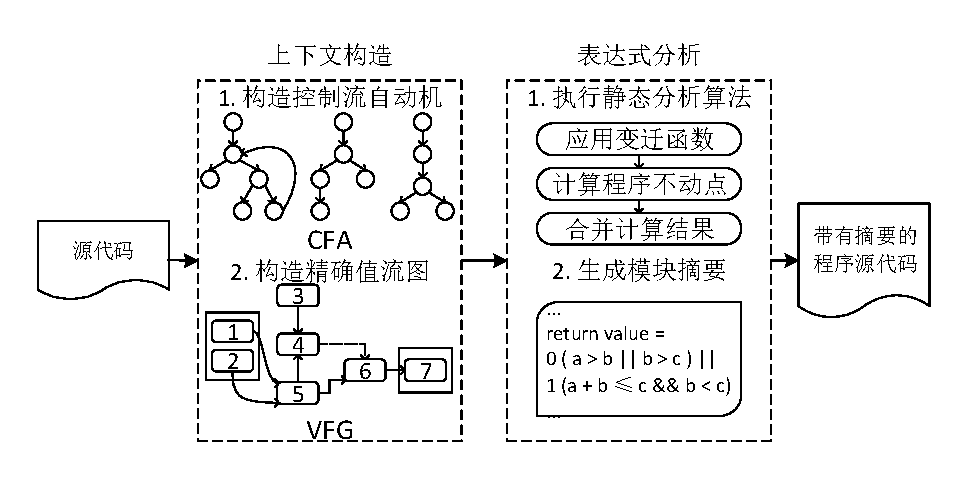
\includegraphics{流程图.pdf}
	\caption{算法的工作流程图}
	\label{fig:流程图}
\end{figure}

\subsection{精确值流图的定义与构造}

在传统的基于控制流图的数据流分析方法中,同一变量在不同路径下的计算结果不同,为了保证算法的正确性,这类算法通常在交汇节点定义状态合并函数,具体使用上近似将变量可能的取值合并。但这将忽略路径信息导致分析精度不足。而精确值流图则是通过内存行为分析与指针别名操作分析,构造出变量取值与数据依赖和控制依赖相结合的值流图。这种精确值流图是路径敏感的,可用来解决状态计算过程中产生的路径丢失问题。

\begin{lstlisting}[label=code:vfgExample,caption=代码样例]
int main() {
	int x = 0, y = 1;
	int *a;
	int p;
	if (p)
		a = &x;
	else
		a = &y;
	return *a;
}
\end{lstlisting}

以代码\ref{code:vfgExample}为例,在第9行的数据流关系为:$ a \gets \{\&x, \&y\} $。而如果使用路径敏感的数据流分析,由于有了路径可达条件信息,可以进一步将a的数据流表示为:$ a \gets \{(\&x, p ≠ 0), (\&y, p = 0)\} $。

\begin{figure}[H]
	\centering
	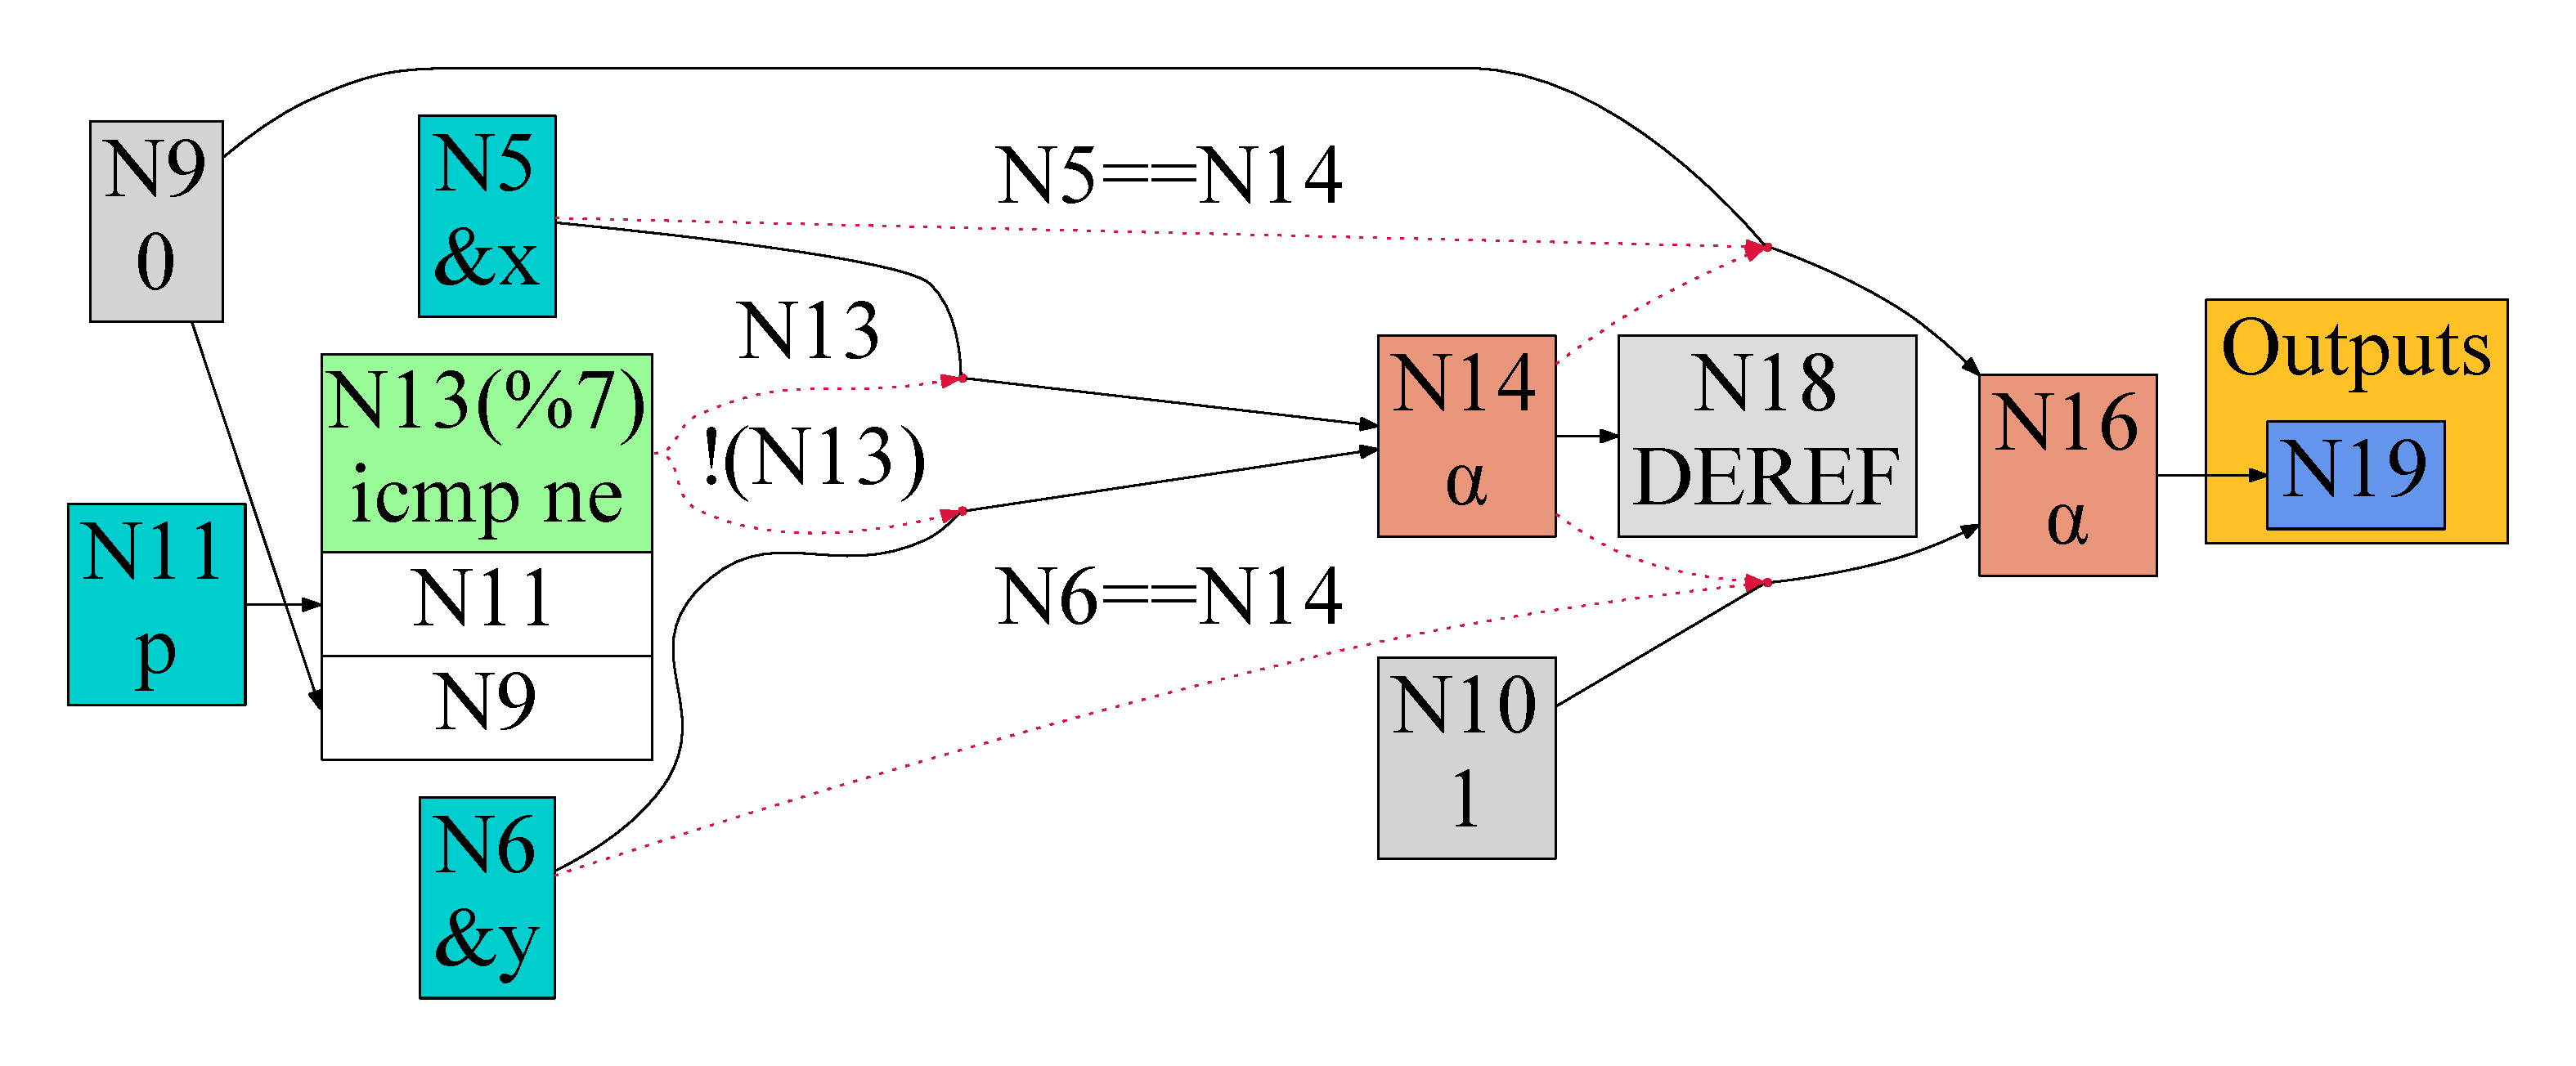
\includegraphics[width=6in]{small.pdf}
	\caption{根据代码\ref{code:vfgExample}生成的值流图}
	\label{fig:small}
\end{figure}

像这样,我们可以把数据流 • ← • 作为值流图上的边,把数据流上承载的数据作为值流图的点,构造值流图如图\ref{fig:small}所示。

值流图按函数划分为不同的值流模块($ Module $),每个$ Module = (N, E) $是一个有向图,其中$ N $是值流图节点集合,每个节点代表程序中的变量或常量。节点$ n ∈ N $上也可以带有条件,表示控制依赖。$ E ⊆ N × N $为有向边集合,表示值的流向。边$ e ∈ E $可以附加条件,表示数据依赖。

我们将VFG的节点按照功能分为如下几类:

常量节点ConstNode:表示程序中的常量,如整数常量、字符串常量、函数指针常量、全局变量的地址常量等,用$ <c> $表示,其中$ c $为字面常量。如图\ref{fig:small}中的节点$ N_{9} $可以表示为$ <0> $。

起始节点StartNode:表示值流图中数据初始化节点,如程序中的变量初始值、参数、函数调用的返回值等等。按照定义可知,起始节点在VFG图中无前驱节点,且该节点不是常量。初始节点用$ <ap> $表示,其中$ ap $是对应的数据的内存位置的访问路径。如图\ref{fig:small}中的节点$ N_{11} $可表示为$ <p> $。

复制节点CopyNode:表示值的复制关系,它的值复制于前驱节点,用$ <n> $表示,其中$ n $是VFG中的节点。如图\ref{fig:small}中的节点$ N_{19} $可表示为$ <N_{16}> $。

运算节点OperatorNode:表示由输入经过运算得到的结果,其中,运算节点以其前驱节点作为运算的输入。运算节点用$ <op, op_1, …, op­_n> $表示,其中$ op $为运算符,$ op_1, …, op­_n $为操作数。这里,操作数即为运算节点的前驱节点。图\ref{fig:small}中节点$ N_{13} $可表示为$ <≠, N_{11}, N_{9}> $。

合并节点JoinNode:合并节点具有多个前驱节点,该节点的取值为前驱节点中的某一个。合并节点用$ <(N_1, C_1), …, (N_i, C_i)> $表示,其中$ N_i $为JoinNode的前驱节点,$ C_i $为数据依赖,表示当$ C_i $为真时,JoinNode的取值为$ N_i $。图\ref{fig:small}中节点$ N_{14} $可表示为$ <(N_5, N_{13}), (N_6, ¬N_{13})> $。

对于每个模块$ M $,定义两个特殊节点集合$ In(M) $和$ Out(M) $分别表示模块的输入节点集合和输出节点集合。其中,输入节点包括函数的参数与全局变量,其类型总是StartNode。而输出节点包括函数的返回值与全局变量,其类型总是CopyNode。

为了便于后续描述算法,我们定义如下函数:
\begin{enumerate}
	\item 定义函数$ literalVal::ConstNode \rightarrow Value $用于取常量节点的具体值;
	\item 定义函数$ symbolicVal::StartNode \rightarrow Value $表示取起始节点的符号值。
\end{enumerate}

\subsection{表达式分析算法}

定义$ ValueCase $为二元组$  (Value, Condition) $,其中$ Value $是值流图上某节点的可能取值,这个值既可以是具体的常量值,如123、“abc”等,又可以是符号表达式,如“a + 3”等;$ Condition $是布尔表达式,它表示当值流图上某节点的$ Condition $条件为真时,其取值为$ Value $。

定义函数$ val::ValueCase \rightarrow Value $表示取$ ValueCase $中$ Value $的值;函数$ cond::ValueCase \rightarrow Condition $表示取$ ValueCase $中$ Condition $的值。

定义抽象函数$ T::Node \rightarrow ValueSet $为从值流图节点到抽象域上的一个映射,其中$ ValueSet $为$ ValueCase $的集合。则基于值流图的表达式分析算法如算法\ref{alg:值流图分析算法}所示。

\begin{algorithm}
[H]
	\caption{值流图分析算法}
	\label{alg:值流图分析算法}
	\begin{algorithmic}[1]
		
		\Require $nodes$: current value flow graph's node set
		
		\State $blockSet \gets \emptyset$
		\State $pending \gets \left\{ n \;|\; n \in nodes, n \text{ is ConstNode or StartNode }\right\}$
		\While{$pending \ne \emptyset$}
		\State $cur \gets $ peek($pending$)
		\State $valueSet \gets$ updateNodeValue($cur$)
		\If{$valueSet = \emptyset$}
		\State $blockSet \gets blockSet \cup cur$
		\ElsIf{$valueSet$ is an update for $cur$}
		\State $pending \gets pending \cup successor(cur)$
		\State move each $node$ from $blockSet$ to $pending$ which is unblocked due to $valueSet$
		\EndIf
		\EndWhile
		
	\end{algorithmic}
\end{algorithm}

其中,函数$ updateNodeValue::Node \rightarrow ValueSet $表示在迭代计算过程中每个节点的计算值,针对不同类型的节点,我们定义不同计算方法,具体计算方法如表\ref{tab:valueUpdate}所示。

\begin{longtable}{cc}
	\caption{各类节点的值的更新算法}
	\label{tab:valueUpdate}  \\ % add \\ command to tell LaTeX to start a new line	
	
	% Appear table header at the first page as well
	\toprule[1.5pt]	
	{\heiti 节点类型} & {\heiti 更新值}  \\
	\midrule[1pt]
	\endfirsthead
	
	% Appear the table header at the top of every page
	\multicolumn{2}{c}{续表~\thetable\hskip1em 各类节点的值的更新算法}\\
	\toprule[1.5pt]	
	{\heiti 节点类型} & {\heiti 更新值}  \\
	\midrule[1pt]
	\endhead 
	
	% Appear \hline at the bottom of every page
	\hline
	\multicolumn{2}{r}{续下页}
	\endfoot 
	\endlastfoot
	
	% data begins here	
	
	ConstNode & $ \left\{ \left( literalVal \left( cur \right), true \right) \right\} $ \\ 
	StartNode & $ \left\{ \left( symbolicVal \left( cur \right), true \right) \right\} $ \\
	CopyNode & $ \left\{ \left(updateNodeValue \left( cur.predecessor \right) \right) \right\} $ \\ 
	OperatorNode &
			$ \left\{ 
					\left( 	\begin{array}{lr}	 		
							operatorValue \\
							\left( opr \left( cur \right), val \left( opd_1 \right), ..., val \left( opd_i \right) \right) \\
							, cond \left( opd_1 \right) \wedge ... \wedge cond \left( opd_i \right) \\
					\end{array} \right)  
			\,\middle\vert\,
					\begin{array}{c}
							opd_i \in T \left( pre_i \right), \\
							pre_i = pred \left( cur \right) \left[ i \right]  
					\end{array}
			\right\} $ \\ 
	JoinNode (Loop) & 
			$ \left\{ \left( \mu, true \right) 
			\,\middle\vert\, 
			\mu \gets \mu \cup val \left( pred \left( cur \right) \right) \right\} $ \\ 
	JoinNode (Normal) & 
			$ \left\{ \left( val \left( pre_i \right), cond \left( pre_i \right) \wedge pcond \left( pre_i \right) \right)
			\,\middle\vert\, 
			pre_i \gets pred_i \left( cur \right) \right\} $ \\ 
	% more data here
	\bottomrule[1.5pt]
\end{longtable}
%
%\begin{table}[htb]
%	\centering
%	\caption{各类节点的值的更新算法}
%	\label{tab:valueUpdatexx}
%	\begin{tabular}{|c|c|}
%		\hline
%		节点类型 & 更新值 \\ \hline
%		ConstNode & $ \left\{ \left( literalVal \left( cur \right), true \right) \right\} $ \\ \hline
%		StartNode & $ \left\{ \left( symbolicVal \left( cur \right), true \right) \right\} $ \\ \hline
%		CopyNode & $ \left\{ \left(updateNodeValue \left( cur.predecessor \right) \right) \right\} $ \\ \hline
%		OperatorNode &
%				$ \left\{ 
%					 		\left( 	\begin{array}{lr}	 		
%							 		operatorValue \\
%							 		\left( opr \left( cur \right), val \left( opd_1 \right), ..., val \left( opd_i \right) \right) \\
%							 		, cond \left( opd_1 \right) \wedge ... \wedge cond \left( opd_i \right) \\
%					 		\end{array} \right)  
%				 		\,\middle\vert\,
%				 				\begin{array}{c}
%				 						opd_i \in T \left( pre_i \right), \\
%				 						pre_i = pred \left( cur \right) \left[ i \right]  
%				 				\end{array}
%				\right\} $ \\ \hline
%		JoinNode (Loop) & 
%				$ \left\{ \left( \mu, true \right) 
%				\,\middle\vert\, 
%				\mu \gets \mu \cup val \left( pred \left( cur \right) \right) \right\} $ \\ \hline
%		JoinNode (Normal) & 
%				$ \left\{ \left( val \left( pre_i \right), cond \left( pre_i \right) \wedge pcond \left( pre_i \right) \right)
%				\,\middle\vert\, 
%				pre_i \gets pred_i \left( cur \right) \right\} $ \\ \hline
%	\end{tabular}
%\end{table}

本算法属于值流图分析算法,定义了两个集合$ pending $和$ blockSet $,分别用于分别用于存储分析算法中待分析的节点和被阻塞的节点。

算法初始化时,将$ blockSet $集合置空,并将所有类型为$ StartNode $和$ ConstNode $的节点置入$ pending $集合中。在每次迭代计算过程中,从$ pending $集合中取出一个节点,如果其前驱节点或数据依赖条件没有计算完成,则将该节点放入$ pending $集合中;否则,按照上表所规定的计算规则对该节点进行计算。如果之前从未对该节点进行过计算,或计算结果与之前不同,则将该节点的全部后继节点放入$ pending $集合中,并检查$ blockSet $中是否有依赖于本次计算结果的节点可被计算,如果有,则将相应节点重新置入$ pending $集合中。根据上述方法,直到所有的节点均被计算完成、并且到达不动点,迭代结束。

\subsection{程序理解与需求确认}
以变速器档位控制代码(代码\ref{code:gearLever})为例,其对应的值流图如图\ref{fig:test-error}所示。

\begin{figure}[H]
	\centering
	\includegraphics[width=6in]{test-error.pdf}
	\caption{根据代码\ref{code:gearLever}生成的值流图}
	\label{fig:test-error}
\end{figure}

应用上述算法对所有节点进行计算,部分节点的计算结果如表\ref{tab:calculationResult}所示。

由于每个模块的输入节点集合$ In(M) $描述了模块所有可能的读入、输出节点集合$ Out(M) $描述了模块所有可能的输出,因此可根据输出输出节点集合构造函数摘要。如图\ref{fig:test-error}所示,由于$ Out(M) $中的节点$ N_{59} $为复制节点,其计算结果与$ N_{56} $相同,因此最终可以得到的模块摘要如表\ref{tab:summaryFromGearLever}第1、2列所示。

摘要清晰的描述了在不同分支路径条件下模块的输入与输出之间的对应关系,从而便于将软件实现与需求文档进行对比,进而提高程序理解与需求确认等工作的效率。另一方面,本算法是一种基于值流图的程序静态分析方法,因此在得到变量表达式关系的同时,可以在其上应用检查规则从而实现代码检查。典型的应用是检查每个节点在不同程序路径下的取值(表达式),判定程序是否存在如除零异常、空指针解引用、多重内存释放等缺陷,提高代码的正确率。

\begin{longtable}{cc}
	\caption{值流图上部分节点的计算结果}
	\label{tab:calculationResult}  \\ % add \\ command to tell LaTeX to start a new line	
	 
	% Appear table header at the first page as well
	\toprule[1.5pt]	
	{\heiti $Node$} & {\heiti $T(Node)$}  \\
	\midrule[1pt]
	\endfirsthead
	
	% Appear the table header at the top of every page
	\multicolumn{2}{c}{续表~\thetable\hskip1em 值流图上部分节点的计算结果}\\
	\toprule[1.5pt]	
	{\heiti $Node$} & {\heiti $T(Node)$}  \\
	\midrule[1pt]
	\endhead 
	
	% Appear \hline at the bottom of every page
	\hline
	\multicolumn{2}{r}{续下页}
	\endfoot 
	\endlastfoot
	
	% data begins here	
	$ N_{4} $ & $ \left\{  \left( x, true \right) \right\} $ \\ 
	$ N_{26} $ & $ \left\{  \left( 690, true \right) \right\} $ \\ 
	$ N_{34} $ & $ \left\{  \left( x > 690, true \right) \right\} $ \\ 
	$ N_{38} $ & $ \left\{  \left( 4, x ≤ 690 \right), \left( 6, x > 690 \right) \right\} $ \\ 
	$ N_{41} $ & $ \left\{  \left( 1, x < 380 \right), \left( 3, 380 ≤ x ≤ 690 \right), \left( 5, x > 690 \right) \right\} $ \\ 
	$ N_{42} $ & $ \left\{  
			\begin{array}{c}
					\left( 0, y ≤ 780 \right), \left( 1, x < 380 \wedge y > 780 \right) , \left( 3, 380 ≤ x ≤ 690 \wedge y > 780 \right) , \\
					\left( 5, x > 690 \wedge y > 780 \right) 
			\end{array}				
			\right\} $ \\ 
	$ N_{56} $ & $ \left\{  
			\begin{array}{c}
					\left( -1, dv ≠ 0 \right), \left( 0, 160 ≤ y ≤780 \wedge dv = 0 \right), \left( 1, x < 380 ∧ y > 780 \wedge dv = 0 \right),  \\
					\left( 2, x < 380 \wedge y < 160 \wedge dv = 0 \right), \left( 3, 380 ≤ x ≤ 690 \wedge y > 780 \wedge dv = 0 \right),  \\
					\left( 4, 380 ≤ x ≤ 690 \wedge y < 160 \wedge dv = 0 \right), \left( 5, x > 690 \wedge y > 780 \wedge dv = 0 \right), \\
					\left( 6, x > 690 \wedge y < 160 \wedge dv = 0 \right),  \\
			\end{array}
			\right\} $ \\ 
	% more data here
	\bottomrule[1.5pt]
\end{longtable}

%\begin{table}[H]
%	\centering
%	\caption{值流图上部分节点的计算结果}
%	\label{tab:calculationResultxx}
%	\begin{tabular}{|c|c|}
%		\hline
%		$Node$ & $T(Node)$ \\ \hline
%		$ N_{4} $ & $ \left\{  \left( x, true \right) \right\} $ \\ \hline
%		$ N_{26} $ & $ \left\{  \left( 690, true \right) \right\} $ \\ \hline
%		$ N_{34} $ & $ \left\{  \left( x > 690, true \right) \right\} $ \\ \hline
%		$ N_{38} $ & $ \left\{  \left( 4, x ≤ 690 \right), \left( 6, x > 690 \right) \right\} $ \\ \hline
%		$ N_{41} $ & $ \left\{  \left( 1, x < 380 \right), \left( 3, 380 ≤ x ≤ 690 \right), \left( 5, x > 690 \right) \right\} $ \\ \hline
%		$ N_{42} $ & $ \left\{  
%				\begin{array}{c}
%						\left( 0, y ≤ 780 \right), \left( 1, x < 380 \wedge y > 780 \right) , \left( 3, 380 ≤ x ≤ 690 \wedge y > 780 \right) , \\
%						\left( 5, x > 690 \wedge y > 780 \right) 
%				\end{array}				
%		\right\} $ \\ \hline
%		$ N_{56} $ & $ \left\{  
%				\begin{array}{c}
%						\left( -1, dv ≠ 0 \right), \left( 0, 160 ≤ y ≤780 \wedge dv = 0 \right), \left( 1, x < 380 ∧ y > 780 \wedge dv = 0 \right),  \\
%						\left( 2, x < 380 \wedge y < 160 \wedge dv = 0 \right), \left( 3, 380 ≤ x ≤ 690 \wedge y > 780 \wedge dv = 0 \right),  \\
%						\left( 4, 380 ≤ x ≤ 690 \wedge y < 160 \wedge dv = 0 \right), \left( 5, x > 690 \wedge y > 780 \wedge dv = 0 \right), \\
%						\left( 6, x > 690 \wedge y < 160 \wedge dv = 0 \right),  \\
%				\end{array}
%		\right\} $ \\ \hline
%	\end{tabular}
%\end{table}

\section{评估与结果}
\label{sec:值流图评估与结果}

\subsection{实验设计}

虑到根据源代码生成精确值流图的过程十分复杂,本算法的实现基于Tsmart静态分析框架,它的优点是使用静态分析的方法,高效的生成控制流自动机和精确值流图。同时该分析框架具有可配置性,能够较容易的获取到所需程序上下文信息,因此我们采用此分析框架,工具的开发语言为Java,工具的框架图如图\ref{fig:架构图}所示。

本节从客观、主观两个方面评估论文算法(工具)在程序理解与需求确认方面的效用。客观评价重点关注算法的完整性与准确性。具体而言,我们考察算法自动生成的摘要质量;主观评价则重点关注工具在具体的生产环境中的可用性与实用性。我们将分别从客观评价和主观评价两个方面对工具进行实验。

\begin{figure}[H]
	\centering
	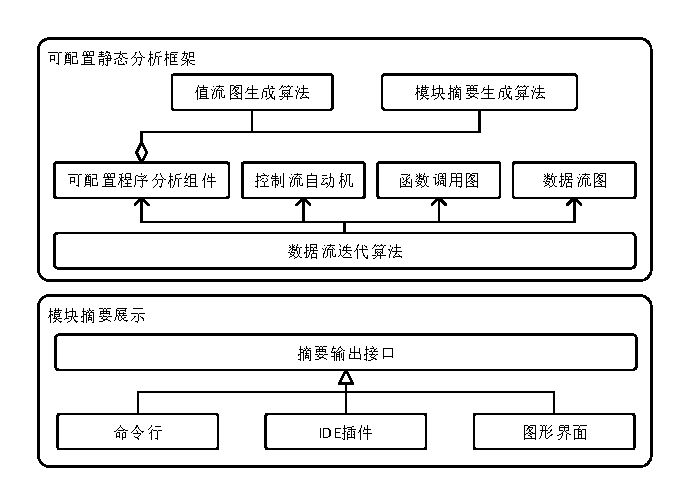
\includegraphics[width=6in]{架构图.pdf}
	\caption{工具架构图}
	\label{fig:架构图}
\end{figure}

\subsection{客观评价}

客观评价方法主要包含以下几个步骤:(1)分别选取数学计算、计算机应用、工业领域和嵌入式领域中8个具有代表性的代码片段作为实验对象(详见表\ref{tab:selectedCodes});(2)采用本文工具分别生成相应的函数摘要;(3)判定工具自动生成的摘要与实际需求的差距。
\begin{longtable}{ccc}
	\caption{选取的各类代码}
	\label{tab:selectedCodes}  \\ % add \\ command to tell LaTeX to start a new line	
	 
	% Appear table header at the first page as well
	\toprule[1.5pt]	
	{\heiti 类别} & {\heiti 选取代码}  & {\heiti 文件名称}  \\
	\midrule[1pt]
	\endfirsthead
	
	% Appear the table header at the top of every page
	\multicolumn{3}{c}{续表~\thetable\hskip1em 选取的各类代码}\\
	\toprule[1.5pt]	
	{\heiti 类别} & {\heiti 选取代码}  & {\heiti 文件名称}  \\
	\midrule[1pt]
	\endhead 
	
	% Appear \hline at the bottom of every page
	\hline
	\multicolumn{3}{r}{续下页}
	\endfoot 
	\endlastfoot
	
	% data begins here	
	\multirow{2}{*}{数学计算} & 三角形判定 & triangle.c \\ 
	& 绝对值计算 & abs.c \\ 
	\multirow{2}{*}{计算机应用} & (加权平均)滤波算法 & filter.c \\ 
	& 校验和算法 & checksum.c \\ 
	\multirow{2}{*}{工业领域} & 车辆控制系统某算法 & CDL\_ARC429.c \\ 
	& 航天发动机控制系统某算法 & ISP\_TOOL.c \\
	\multirow{2}{*}{嵌入式领域} & 含goto语句的程序片段 & msp430-decode.c \\
	& 带函数指针的程序片段 & xen-ops.c \\ 
	% more data here
	\bottomrule[1.5pt]
\end{longtable}
%\begin{table}[htb]
%	\centering
%	\caption{选取的各类代码}
%	\label{tab:selectedCodesxx}
%	\begin{tabular}{|c|c|c|}
%		\hline
%		类别 & 选取代码 & 文件名称 \\ \hline
%		\multirow{2}{*}{数学计算} & 三角形判定 & triangle.c \\ \cline{2-3} 
%		& 绝对值计算 & abs.c \\ \hline
%		\multirow{2}{*}{计算机应用} & (加权平均)滤波算法 & filter.c \\ \cline{2-3} 
%		& 校验和算法 & checksum.c \\ \hline
%		\multirow{2}{*}{工业领域} & 车辆控制系统某算法 & CDL\_ARC429.c \\ \cline{2-3} 
%		& 航天发动机控制系统某算法 & ISP\_TOOL.c \\ \hline
%		\multirow{2}{*}{嵌入式领域} & 含goto语句的程序片段 & msp430-decode.c \\ \cline{2-3} 
%		& 带函数指针的程序片段 & xen-ops.c \\ \hline
%	\end{tabular}
%\end{table}

由于摘要结果和程序的条件分支有关,因此本文分别对比两者在每个条件分支下的生成结果。同时,记录工具的时间和空间开销,包括摘要生成时间、占用内存大小以及生成的VFG大小,如表\ref{tab:summaryComparision}所示。

\begin{table}[htb]
	\centering
	\caption{自动生成摘要和人工生成摘要的对比}
	\label{tab:summaryComparision}
	\begin{tabular}{|c|c|c|c|c|c|c|c|}
		\hline
		\multicolumn{2}{|c|}{程序代码} & 实际需求 & \multicolumn{4}{c|}{自动摘要} & \multirow{2}{*}{\begin{tabular}[c]{@{}c@{}}正确\\ 率\end{tabular}} \\ \cline{1-7}
		类型 & 代码行 & 分支数 & 分支数 & 耗时/s & 内存/MB & VFG大小/KB &  \\ \hline
		三角形判定 & 24 & 4 & 4 & 3 & 134 & 9 & 1.0 \\ \hline
		绝对值 & 11 & 2 & 2 & 2 & 122 & 2 & 1.0 \\ \hline
		滤波算法 & 19 & 1 & 1 & 2 & 128 & 4 & 1.0 \\ \hline
		校验和算法 & 22 & 1 & 1 & 2 & 145 & 12 & 1.0 \\ \hline
		车辆控制系统 & 124 & 12 & 12 & 5 & 167 & 53 & 1.0 \\ \hline
		航发控制系统 & 178 & 15 & 15 & 6 & 171 & 61 & 1.0 \\ \hline
		Goto语句 & 57 & 8 & 8 & 4 & 137 & 34 & 1.0 \\ \hline
		函数指针 & 36 & 3 & 3 & 3 & 132 & 6 & 1.0 \\ \hline
	\end{tabular}
\end{table}

经实验验证,本工具能够完整地生成不同类型代码的摘要,且生成摘要的条件分支数与需求一致。运行工具所消耗的资源相对较少,内存占用小于200MB,生成的VFG均小于1MB。工具可以较快的生成函数摘要,生成百行级别代码所需时间不超过1分钟。

\subsection{主观评价}

为保证主观评价的公平性与准确性,现从学校选取共30名条件相当的同学参与实验,他们均符合以下条件:(1)拥有超过3年的C语言编程经验,且均使用C语言通过了学校的编程水平测验;(2)对表\ref{tab:selectedCodes}代码所在的背景了解程度相当。

实验方法包含以下几个步骤:(1)将30名同学分为源码组和摘要组进行对照实验,分别为其提供表5所示的8份源代码(或含摘要的源代码);(2)令每名同学阅读代码,并令其说出代码功能,记录用时T1;(3)令每名同学分析函数在不同输入的情况下的输出,记录用时T2;(4)分别统计并对比两组同学在不同代码上回答问题所用时间T1和T2的平均值;(5)在源码组同学完成后,为其提供摘要。同时分别询问两组同学对摘要的看法。 

如表\ref{tab:ComprehensionComparision}所示为两组同学在各个代码上回答实验步骤2和3中提出问题的平均用时T1和T2。通过对比可知,在代码行数较小(10行以内)且逻辑并不复杂的情况下,使用摘要对程序理解无明显帮助。但当面对几十甚至上百行代码时,使用摘要可明显减少用户理解代码所用时间。在含goto语句的实验样本上,可节省60.5\%的程序理解时间。

通过实验可知,本工具可显著提高用户对代码的理解效率,能够帮助用户快速抽取程序语义并进行需求确认。同时,随着代码分支复杂度的提升,使用工具进行程序理解与需求确认的优势将越来越大。

\begin{longtable}{ccccc}
	\caption{各组对每类代码理解并作答所用时间}
	\label{tab:ComprehensionComparision}  \\ % add \\ command to tell LaTeX to start a new line	

	% Appear table header at the first page as well
	\toprule[1.5pt]	
	{\heiti 程序代码} & {\heiti 源码组T1/s}  & {\heiti 源码组T2/s}  & {\heiti 摘要组T1/s}  & {\heiti 摘要组T2/s}    \\
	\midrule[1pt]
	\endfirsthead
	
	% Appear the table header at the top of every page
	\multicolumn{5}{c}{续表~\thetable\hskip1em 选取的各类代码}\\
	\toprule[1.5pt]	
	{\heiti 程序代码} & {\heiti 源码组T1/s}  & {\heiti 源码组T2/s} & {\heiti 摘要组T1/s}   & {\heiti 摘要组T2/s}    \\
	\midrule[1pt]
	\endhead 
	
	% Appear \hline at the bottom of every page
	\hline
	\multicolumn{5}{r}{续下页}
	\endfoot 
	\endlastfoot
	
	% data begins here	
	三角形判定 & 45 & 32 & 37 & 14 \\ 
	绝对值 & 5 & 13 & 11 & 14 \\ 
	滤波算法 & 61 & 15 & 27 & 15 \\ 
	校验和算法 & 97 & 43 & 54 & 38 \\ 
	车辆控制系统 & 294 & 86 & 103 & 74 \\ 
	航发控制系统 & 318 & 92 & 114 & 91 \\ 
	Goto语句 & 195 & 48 & 64 & 31 \\ 
	函数指针 & 82 & 33 & 40 & 29 \\ 
	% more data here
	\bottomrule[1.5pt]
\end{longtable}
%\begin{table}[htb]
%	\centering
%	\caption{各组对每类代码理解并作答所用时间}
%	\label{tab:ComprehensionComparisionxx}
%	\begin{tabular}{|c|c|c|c|c|}
%		\hline
%		程序代码 & 源码组T1/s & 源码组T2/s & 摘要组T1/s & 摘要组T2/s \\ \hline
%		三角形判定 & 45 & 32 & 37 & 14 \\ \hline
%		绝对值 & 5 & 13 & 11 & 14 \\ \hline
%		滤波算法 & 61 & 15 & 27 & 15 \\ \hline
%		校验和算法 & 97 & 43 & 54 & 38 \\ \hline
%		车辆控制系统 & 294 & 86 & 103 & 74 \\ \hline
%		航发控制系统 & 318 & 92 & 114 & 91 \\ \hline
%		Goto语句 & 195 & 48 & 64 & 31 \\ \hline
%		函数指针 & 82 & 33 & 40 & 29 \\ \hline
%	\end{tabular}
%\end{table}

在实验步骤5中,我们设计了数道问题,交予参与实验的同学回答并统计,最终得到的结果如表\ref{tab:questionaire}。实验参与者对自动生成摘要工具总体持肯定态度,认为生成的摘要对理解代码有帮助。对于摘要是否可以帮助分析变更影响范围与帮助软件维护方面,一部分同学持观望和怀疑态度,认为本工具生成的摘要为函数级别的摘要,而变更影响范围分析与软件维护可能涉及全局代码,需要结合函数调用等信息进一步分析。

\begin{longtable}{cccc}
	\caption{问卷设计与答复情况}
	\label{tab:questionaire}  \\ % add \\ command to tell LaTeX to start a new line	
	
	% Appear table header at the first page as well
	\toprule[1.5pt]	
	{\heiti 问题设计} & {\heiti 赞同人数}  & {\heiti 否定人数}  & {\heiti 其他想法}  \\
	\midrule[1pt]
	\endfirsthead
	
	% Appear the table header at the top of every page
	\multicolumn{4}{c}{续表~\thetable\hskip1em 问卷设计与答复情况}\\
	\toprule[1.5pt]	
	{\heiti 问题设计} & {\heiti 赞同人数}  & {\heiti 否定人数}  & {\heiti 其他想法}  \\
	\midrule[1pt]
	\endhead 
	
	% Appear \hline at the bottom of every page
	\hline
	\multicolumn{4}{r}{续下页}
	\endfoot 
	\endlastfoot
	
	% data begins here	
	摘要是否有助于你理解代码? & 28 & 2 & 0 \\
	你认为摘要是否对影响范围分析有帮助? & 25 & 4 & 1 \\ 
	你认为摘要是否对软件维护有帮助? & 22 & 7 & 1 \\ 
	% more data here
	\bottomrule[1.5pt]
\end{longtable}
%\begin{table}[htb]
%	\centering
%	\caption{问卷设计与答复情况}
%	\label{tab:questionairexx}
%	\begin{tabular}{|c|c|c|c|}
%		\hline
%		问题设计 & 赞同人数 & 否定人数 & 其他想法 \\ \hline
%		摘要是否有助于你理解代码? & 28 & 2 & 0 \\ \hline
%		你认为摘要是否对影响范围分析有帮助? & 25 & 4 & 1 \\ \hline
%		你认为摘要是否对软件维护有帮助? & 22 & 7 & 1 \\ \hline
%	\end{tabular}
%\end{table}

\section{后续工作与总结}
\label{sec:值流图总结}

本方法依赖于精确值流图的准确生成,当前可用工具相对较少,且在面对大型程序时消耗的时间空间较多。这会对本工具的结果造成一定影响。一个可能的解决方案是在原有的值流图算法上进行优化,针对于循环与数组,优化其结果。

另一方面,为了保证算法的收敛性与时间开销,本算法在处理循环时,引入了符号值$ \mu $,算法的结果是带$ \mu $的符号表达式,这将在处理循环时带来一定的精度丢失。后续可以使用循环不变式等技术进一步提高分析精度。同时,为了增强工具对全局影响范围的分析,后续将会结合函数调用等信息,提升工具的适用性。

软件验证与维护是软件研发中不可或缺的一环,而提高研发者对程序的理解速度则是其中的关键所在。传统的技术和工具或者难以有效帮助程序员减少代码阅读量,或者具有较高的使用门槛,难以广泛使用。本文的研究工作试图针对这一问题,提供一个程序理解算法与摘要生成工具。

本章首先通过一个变速器档位控制逻辑的案例剖析了程序理解对软件开发的重要性,并借此提出函数摘要的作用。随后介绍相关程序理解方法与摘要生成算法。我们在可配置的静态分析框架上实现了摘要生成算法,并从内外两个方面结合实验证明了摘要生成算法的有效性与实用性。

尽管本章提出的方法具有一定的局限性,但本章的研究结果仍可对程序理解、变量表达式分析和程序变更影响分析工具的设计与实现提供思路和指导。